\documentclass[a4paper]{report}
\usepackage[14pt]{extsizes}
\usepackage[utf8]{inputenc}
\usepackage[english,russian]{babel}
\usepackage[OT1]{fontenc}
\usepackage{setspace, amsmath}
\usepackage{amsfonts}
\usepackage{amssymb}
\usepackage[left=20mm, top=10mm, right=15mm, bottom=20mm, nohead, footskip=10mm]{geometry}
\usepackage{gensymb}
\usepackage{alltt}
\addto\captionsrussian{\def\refname{Ссылки}}
\bibliographystyle{gost780u}

\usepackage{graphicx} 
\graphicspath{{images/}}
\DeclareGraphicsExtensions{.pdf,.png,.jpg}

\renewcommand{\theenumi}{\arabic{enumi}}
\renewcommand{\labelenumi}{\arabic{enumi}}
\renewcommand{\theenumii}{.\arabic{enumii}}
\renewcommand{\labelenumii}{\arabic{enumi}.\arabic{enumii}.}
\renewcommand{\theenumiii}{.\arabic{enumiii}}
\renewcommand{\labelenumiii}{\arabic{enumi}.\arabic{enumii}.\arabic{enumiii}.}
\usepackage{indentfirst}
\usepackage{fontspec}
\setmainfont{Times New Roman}

\begin{document}
\begin{titlepage}
\newpage



\begin{center}
\vfill
%\framepage

Федеральное государственное бюджетное образовательное учреждение высшего образования «МИРЭА — Российский технологический университет»\\
\ \\

\hfill\vbox
{
\hbox{базовая кафедра № 252}
}

\vfill

{\large\bf Разработка безопасного аудиокодека с шифрованием трафика\\}
\ \\
Реферат студентов 1 курса института искусственного интеллекта\\
Коровяковского Степана и Урвачева Романа

\vfill

%{
%\hbox{Научный руководитель:}
%\hbox to 16cm {к.т.н, доцент \hrulefill Х.З.~Мамаев}
%\hbox{}
%\hbox{Заведующий кафедрой:}
%\hbox to 16cm {д.ф.-м.н., профессор \hrulefill В.С.~Луговской}
%}

\vfill

Москва 2022
\end{center}

\end{titlepage}
\tableofcontents
\newpage
%\chapter*{Введение}
%Данная работа разделена на 4 главы. В первой главе будут рассмотрены способы передачи аудиоинформации в целом. Во второй главе будут описаны алгоритмы сжатия данных. А в третьей главе будут приведены алгоритмы блочного и поточного шифрования данных.

\chapter{Изучение способов передачи аудиоданных в информационно-телекоммуникационных сетях}
\section{Телекоммуникационные технологии}
Каждому поколению свойственно разрабатывать новые технические средства, совершенствовать систему учета, обработки, передачи и хранения данных. Первыми телекоммуникационными средствами признан телеграф, телефон, телетайп, радиоприемник. Середина XIX столетия отмечена массовым использованием спутниковой связи, вычислительной техники, компьютерной сети. В результате это положительно отразилось на развитии новых телекоммуникационных технологий.
\par Современный мир невозможен без телекоммуникационных технологий, которые стирают государственные границы и расстояние между людьми, делают доступной мобильную и видеосвязь и позволяют решать множество задач в сфере управления, образования, коммерции. Каждый человек сталкивается с ними ежедневно, деля телефонные звонки, проверяя почту или покупая товары в интернет-магазинах.

\subsection{Определение и понятие телекоммуникационных \\ технологий}
Общее понятие информационных и коммуникационных технологий включает в себя совокупность методов, процессов и устройств, позволяющих получать, собирать, накапливать, хранить, обрабатывать и передавать информацию, закодированную в цифровом виде или существующую в аналоговом виде.
\par В более узком смысле под телекоммуникационными технологиями понимается совокупность программных и аппаратных средств, позволяющих устанавливать связь без использования проводов и передавать пакеты информации.

\subsection{Виды телекоммуникационных технологий}
Телекоммуникационные технологии могут быть рассмотрены как сервисы, предоставляемые провайдерами различного уровня.
По этому принципу можно выделить следующие виды телекоммуникационных технологий:
\begin{itemize}
\item телефонная связь, современная телефонная связь позволяет легко переключаться с аналогового стандарта на цифровой, подключать к интернет городские телефоны и соединять в одну сеть аналоговые и мобильные устройства;
\item радиосвязь, которая сегодня превратилась в сотовую связь, телефон, перемещаясь в пределах сети, оказывается в зоне действия различных передающих устройств;
\item спутниковая связь, которая используется провайдерами для создания систем мобильной связи и для государственных систем связи;
\item интернет – наиболее распространенный вид телекоммуникационных технологий, при которых подключение к сети может осуществляться как проводным, так и беспроводным способом.
\end{itemize}

\subsection{Основные типы информационно-телекоммуникационных сетей}
Телекоммуникационные технологии, используемые в интернете, сейчас переживают этап бурного развития и роста. С каждым днём создаётся всо больше и больше новых сетей различных типов, среди которых основными являются:
\begin{itemize}
\item локальные сети компаний или учреждений (Local Area Network - LAN), связь между компьютерами в них осуществляется и проводным и беспроводным способом, количество пользователей этих сетей ограничено. Локальные сети могут быть корпоративными, в некоторых странах создаются и городские локальные сети;
\item глобальные сети (Wide Area Network – WAN) представляют совокупность большого количества узлов-компьютеров, расположенных в разных странах мира и связанных между собой каналами оптово-волоконной связи. К этим сетям, представляющим услуги провайдеров, подключаются локальные сети.
\end{itemize}

\subsection{Технические и программные средства \\ телекоммуникационных технологий}
Работоспособность интернета основана на использовании сетевых узлов и каналов связи. К узлам относятся как отдельные компьютеры, так и хостинги, предоставляющие IP-адреса и доменные имена.
Каналы связи делятся на 4 типа:
\begin{itemize}
\item аналоговые телефонные сети;
\item провода, по которым передается электричество;
\item оптоволоконные каналы связи;
\item беспроводные каналы связи, модемные или спутниковые.
\end{itemize}
К телекоммуникационным каналам связи относятся, в основном, третий и четвертый типы.

Среди коммуникаций, используемых для организации связи, можно отдельно отметить программы, обеспечивающие работу телекоммуникационного оборудования такого, как:
\begin{itemize}
\item IP-АТС;
\item маршрутизаторы;
\item компьютеры.
\end{itemize}

\subsection{Основные задачи сетевых телекоммуникационных \\ технологий}
Различные сетевые телекоммуникационные технологии позволяют решать такие задачи, как:
\begin{itemize}
\item передачу информации в необходимых форматах;
\item выстраивание коммуникаций;
\item обеспечение взаимодействия различных участников сети.
\end{itemize}

Среди новых технологий особое место занимают программы, позволяющие работать в режиме нетворкинга, объединение CRM-систем с возможностями социальных сетей и многое другое.

Создание корпоративных сетей как офисных, компьютерных, так и телефонных, также попадает в область сетевых технологий, призванных обеспечить синергию за счет эффективной коммуникации пользователей.

~

Спектр возможностей использования телекоммуникационных технологий расширяется с каждым днем. Сложно сказать, что именно будет предложено завтра в этой области, чтобы сделать связь доступнее, а производственные процессы – проще.

\section{Описание способов передачи аудиоданных}
\subsection{Передача аудиоданных по телефонным каналам связи}

Взаимное проникновение вычислительной техники и технических средств связи оказало серьезное влияние как на структуру компьютеров, так и на структуру каналов связи.

Средства связи, предназначенные для передачи информации между людьми, имеют длительную историю, развитую структуру (в мировом масштабе), мощную научную и технологическую базу и, начиная с 60-х годов, стали использоваться для передачи данных, т.е. для передачи информации между техническими средствами вычислительной техники, что потребовало включения в каналы связи дополнительных технических устройств.

В настоящее время для распределенных вычислительных систем наиболее широко используются телефонные каналы.

На рис. 1.2.1.1 представлена упрощенная схема линии аналоговой междугородней телефонной связи.

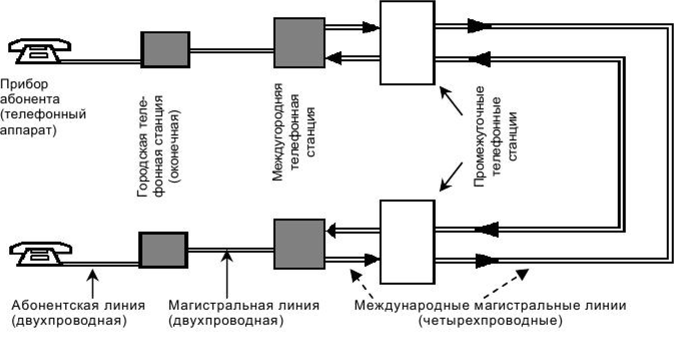
\includegraphics[scale=1.4]{66}
{\centering\caption{Рис. 1.2.1.1 Схема междугородней телефонной связи}\\}
~

На участке от телефонного аппарата до местной АТС происходит передача в первичной полосе частот « 200 - 3100 Гц (полоса частот человеческого голоса). При этом от каждого аппарата до АТС проводится двухпроводная электрическая линия для передачи этого сигнала, в дальнейшем происходит преобразование его в иную форму с целью уплотнения передачи. В каждом из последующих каналов идет очень большое количество передач. Существует два типа уплотнения: частотное и временное. В традиционных линиях связи, как правило, используется частотное уплотнение.

\subsubsection{Описание типов каналов связи}

В зависимости от типа передачи различают аналоговые (традиционно используемые, имеющие длительную историю развития) и цифровые каналы (систем ИКМ, ШОЫ и др.), являющиеся битовым трактом с цифровым импульсным сигналом на выходе и входе канала. Цифровые каналы отличаются рядом преимуществ перед аналоговыми, поэтому вновь создаваемые системы передачи данных стараются строить на основе цифровых каналов. Следует отметить, что цифровые каналы весьма успешно применяются не только для передачи данных, но и в средствах бытовой связи (звук, изображение и г.д.), при этом аналоговые сигналы кодируются в цифровые перед передачей в канал.

Термины «аналоговый» и «цифровой» соответствуют непрерывным и дискретным процессам и используются при обсуждении коммуникационных систем в различных контекстах - данных, сигналов и передачи.

Аналоговые данные представляются физической величиной, которая может изменяться в непрерывном диапазоне значений. Величина прямо пропорциональна данным или является их функцией.

Цифровые данные принимают дискретные значения - текст, целые числа, двоичные данные.

Аналоговый сигнал - непрерывно изменяющаяся электромагнитная волна, распространяющаяся в различных средах.

Цифровой сигнал - дискретный (разрывной) сигнал, такой, как последовательность импульсов напряжения.

Возможны четыре вида передачи данных:
\begin{enumerate}
\item) цифровые данные - цифровой сигнал, используется наиболее простое оборудование;
\item) аналоговые данные - цифровой сигнал, необходимо преобразование аналоговых данных в цифровую форму, что позволяет использовать современное (высокоэффективное) оборудование передачи данных;
\item) цифровые данные - аналоговый сигнал, необходимость преобразования связана с тем, что через некоторые среды (оптоволокно, беспроводные среды) может распространяться только аналоговый сигнал;
\item) аналоговые данные - аналоговый сигнал, традиционная передача, аналоговые данные легко преобразуются в аналоговый сигнал.
\end{enumerate}
\subsubsection{Основные преимущества цифровой передачи данных}
Среди преимуществ цифровой передачи необходимо отметить следующие.
\begin{itemize}
\item \qquad Быстрое развитие цифровых систем и уменьшение цены и размеров оборудования, цены и размеры аналогового оборудования остаются на прежнем уровне. Обслуживание цифровых систем намного дешевле аналоговых.
\item \qquad Использование повторителей (в цифровых системах) вместо аналоговых усилителей позволяет передавать данные на большие расстояния по менее качественным линиям (нет накопления шумов) - сохранение целостности данных.
\item \qquad Большая пропускная способность дает возможность более полно использовать пропускную способность оптоволокна и спутниковых средств связи. Временное разделение оказывается более эффективным, чем частотное.
\item \qquad Используется интеграция, когда при обработке аналоговой и цифровой информации по цифровым технологиям все сигналы имеют одинаковую форму (вид). Эго позволяет сэкономить на оборудовании и трудозатратах при интеграции: голос, видео, цифровые данные.
\end{itemize}
\subsubsection{Модемы}
Термин «модем» применяется в настоящие время (в связи с распространением цифровых каналов) достаточно широко, при этом необязательно подразумевается какая-либо модуляция, а просто называются определенные операции преобразования сигналов, поступающих от ЭТЕ для их дальнейшей передачи по используемому каналу.

Существует очень много разновидностей модемов, отличающихся:
\begin{itemize}
\item по конструкции - внутренние (вставляемые в разъемы компьютера) и внешние, портативные, групповые и т.н.;
\item по методу передачи - асинхронные, синхронные, синхронноасинхронные.
\end{itemize}

Асинхронный метод передачи (или стартстопный) - посимвольный режим передачи с контролем начала и конца символа, имеет низкую скорость и малую эффективность. Синхронный метод передачи осуществляет объединение большого количества символов или байт в отдельные блоки - кадры, которые передаются без задержек между восьмибитными элементами.

~

\subsubsection{Режимы работы в зависимости от направления передачи}
Очень важной характеристикой канала передачи являются режимы его работы в зависимости от направления возможной передачи данных:
\begin{itemize}
\item симплексный - передача осуществляется по линии связи только в одном направлении;
\item полудуплексный - передача ведется в обоих направлениях, но попеременно во времени (технология Ethernet);
\item дуплексный - передача ведется одновременно в двух направлениях.
\end{itemize}

Дуплексный режим - наиболее универсальный и производительный. Самым простым вариантом организации дуплексного режима является использование двух независимых функциональных каналов (двух пар проводников или двух световодов) в кабеле, каждый из которых работает в симплексном режиме, т.е. передает данные в одном направлении. Такая организация дуплексного режима применяется во многих сетевых технологиях (Fast Ethernet, ATM и т.п.).

\subsection{Передача аудиоданных по радиосвязи}

Радиосвязь – быстрый и относительно надежный способ передачи данных на большие расстояния. При этом нет необходимости в использовании физического носителя, например проводов.

Свойства волн разной длины напрямую влияют на их применение для обеспечения радиосвязи. Кроме того, на качество передачи информации с их помощью влияют следующие факторы:

\begin{itemize}
\item высота приемной и передающей антенн;
\item рельеф поверхности;
\item солнечная активность, метеоусловия, время суток.
\end{itemize}

\subsubsection{Процесс приема-передачи информации}

Процесс приема-передачи информации с помощью радиоволн состоит из следующих основных этапов:

\begin{enumerate}

\item) формирование сигнала;
\item) выделение несущей частоты;
\item) связывание передаваемой информации с несущей частотой (модуляция);
\item) трансформация сигнала в дискретный вид, его кодирование (для цифровых систем);
\item) передача в радиоэфир с помощью антенны;
\item) прием сигнала;
\item) декодировка и демодуляция;
\item) преобразование сигнала в форму понятную абоненту.
\end{enumerate}

\subsubsection{Оборудование для осуществления передачи данных}
Чтобы реализовать обмен информации необходимо чтобы у принимающей и передающей стороны в наличии было следующее оборудование:

\begin{itemize}
\item передатчик;
\item антенна;
\item ретрансляционное устройство – позволяет увеличить дальность передачи сигнала;
\item принимающее устройство;
\item оборудование модуляции-демодуляции, сжатия, оцифровки и кодирования;
\item фильтры помех, усилители.
\end{itemize}

\subsubsection{Способы передачи данных по радиосвязи}
Применяется несколько способов радиосвязи, для каждого из которых используется специфическое оборудование. Три наиболее распространенных вида:
\begin{itemize}
\item сотовая связь;
\item радиорелейная связь;
\item спутниковая связь.
\end{itemize}


\subsubsection{Сферы применения радиосвязи}

Возможность практически мгновенной передачи информации на любые расстояния создает широкие возможности использования во всех сферах деятельности человека. Радиосвязь успешно применяется в следующих отраслях:

\begin{itemize}
\item телевизионное и радиовещание;
\item качественная связь по безопасным линиям востребована в военной отрасли. Позволяет осуществлять управление и координацию боевых подразделений;
\item в области транспорта – обеспечивается постоянная связь с поездами, морскими и речными судами, самолетами, грузовыми и легковыми автомобилям (полиция, скорая помощь, такси, курьерские службы);
\item организация диспетчерских служб;
\item обеспечение различных видов коммуникации: спутниковая, мобильная связь;
\item беспроводное подключение к сети Интернет.
\end{itemize}

Также широкие возможности коммуникации являются неотъемлемым инструментом практически любого современного бизнеса. При помощи беспроводной связи можно успешно решать вопросы управления удаленными объектами.


\subsection{Передача аудиоданных через системы спутниковой связи}

Системы спутниковой связи (ССС) широко используются во многих регионах мира и стали неотъемлемой частью инфраструктуры телекоммуникаций большинства стран. Не только промышленно развитые страны с разнообразными современными сетями телекоммуникаций, но все чаще и развивающиеся страны успешно внедряют ССС. 

Новые спутниковые приложения обеспечивают быстрое создание новых широковещательных служб и частных сетей.



\subsubsection{Устройство спутниковой связи}
Спутник - устройство связи, которое принимает сигналы от земной станции (ЗС), усиливает и транслирует в широковещательном режиме одновременно на все ЗС, находящиеся в зоне видимости спутника. Спутник не инициирует и не терминирует никакой пользовательской информации за исключением сигналов контроля и коррекции возникающих технических проблем и сигналов его позиционирования. Спутниковая передача начинается в некоторой ЗС, проходит через спутник, и заканчивается в одной или большем количестве ЗС.

ССС состоит из трех базисных частей: космического сегмента, сигнальной части и наземного сегмента (рис. 1.2.3.1). Космический сегмент охватывает вопросы проектирования спутника, расчета орбиты и запуска спутника. Сигнальная часть включает вопросы используемого спектра частоты, влияния расстояния на организацию и поддержание связи, источники интерференции сигнала, схем модуляции и протоколов передачи. Наземный сегмент включает размещение и конструкцию ЗС, типы антенн, используемых для различных приложений, схемы мультиплексирования, обеспечивающие эффективный доступ к каналам спутника.

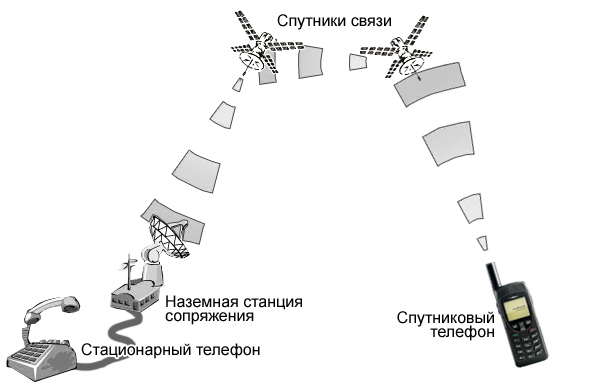
\includegraphics[scale=0.7]{70}
{\centering\caption{\newline Рис. 1.2.3.1}\\}

~

На рис. 1.2.3.1: космический сегмент - спутники связи, сигнальная часть - наземная станция сопряжения, наземный сегмент - спутниковый телефон.

\subsubsection{Преимущества и ограничения систем спутниковой связи}
Системы спутниковой связи имеют уникальные особенности, отличающие их от других систем связи. Некоторые особенности обеспечивают преимущества, делающие спутниковую связь привлекательной для ряда приложений. Другие создают ограничения, которые неприемлемы при реализации некоторых прикладных задач.

ССС имеет ряд преимуществ:
\begin{itemize}
\item Устойчивые издержки. Стоимость передачи через спутник по одному соединению не зависит от расстояния между передающей и принимающей ЗС. Более того, все спутниковые сигналы - широковещательные. Стоимость спутниковой передачи, следовательно, остается неизменной независимо от числа принимающих ЗС.
\item Широкая полоса пропускания.
\item Малая вероятность ошибки. В связи с тем, что при цифровой спутниковой передаче побитовые ошибки весьма случайны, применяются эффективные и надежные статистические схемы их обнаружения и исправления.
\end{itemize}

Выделим также ряд ограничений в использовании ССС:

\begin{itemize}
\item Значительная задержка. Большое расстояние от ЗС до спутника на геосинхронной орбите приводит к задержке распространения, длиной почти в четверть секунды. Эта задержка вполне ощутима при телефонном соединении и делает чрезвычайно неэффективным использование спутниковых каналов при неадаптированной для ССС передаче данных.
\item Размеры ЗС. Крайне слабый на некоторых частотах спутниковый сигнал, доходящий до ЗС (особенно для спутников старых поколений), заставляет увеличивать диаметр антенны ЗС, усложняя тем самым процедуру размещения станции.
\item Защита от несанкционированного доступа к информации. Широковещание позволяет любой ЗС, настроенной на соответствующую частоту, принимать транслируемую спутником информацию. Лишь шифрование сигналов, зачастую достаточно сложное, обеспечивает защиту информации от несанкционированного доступа.
\item Интерференция. Спутниковые сигналы, действующие в Ku- или Ka-полосах частот (о них ниже), крайне чувствительны к плохой погоде. Спутниковые сети, действующие в C-полосе частот, восприимчивы к микроволновым сигналам. Интерференция вследствие плохой погоды ухудшает эффективность передачи в Ku- и Ka-полосах на период от нескольких минут до нескольких часов. Интерференция в С-полосе ограничивает развертывание ЗС в районах проживания с высокой концентрацией жителей.
\end{itemize}

Влияние упомянутых преимуществ и ограничений на выбор спутниковых систем для частных сетей довольно значительно. Решение об использовании ССС, а не распределенных наземных сетей, всякий раз необходимо экономически обосновать.


\subsubsection{Роль наземного сегмента}
Технологическое развитие привело к значительному уменьшению размеров земных сегментов. На начальном этапе спутник не превышал нескольких сотен килограммов, а ЗС представляли собой гигантские сооружения с антеннами более 30 м в диаметре. Современные спутники весят несколько тонн, а антенны, зачастую не превышающие 1 м в диаметре, могут быть установлены в самых разнообразных местах. Тенденция уменьшения размеров ЗС вместе с упрощением установки оборудования приводит к снижению его стоимости. На сегодняшний день стоимость ЗС является, пожалуй, главной характеристикой, определяющей широкое распространение ССС. Преимущество спутниковой связи основано на обслуживании географически удаленных пользователей без дополнительных расходов на промежуточное хранение и коммутацию. Любые факторы, понижающие стоимость установки новой ЗС, однозначно содействуют развитию приложений, ориентированных на использование ССС.

~

Последние достижения технологии в области спутниковой связи говорят о больших потенциальных возможностях ССС в расширении пропускной способности каналов передачи, разработке и внедрении новых служб связи. Будущее ССС за широкополосными широковещательными приложениями и спутниковыми системами подвижной связи.


\subsection{Передача аудиоданных через Интернет}
Аудио через IP — распространение цифрового аудио по IP-сети, такой как Интернет. Все чаще используется для обеспечения высококачественной передачи звука на большие расстояния.

\subsubsection{IP - телефония}

IP-телефония — телефонная связь по протоколу IP. Под IP-телефонией подразумевается набор коммуникационных протоколов, технологий и методов, обеспечивающих традиционные для телефонии набор номера, дозвон и двустороннее голосовое общение, а также видеообщение по сети Интернет или любым другим IP-сетям. Сигнал по каналу связи передаётся в цифровом виде и, как правило, перед передачей преобразовывается, чтобы удалить избыточность информации и снизить нагрузку на сеть передачи данных.

~

Самая главная особенность рассматриваемой связи — это то, что передача информации происходит не по специально выделенным телефонным линиям, а через компьютерную сеть. Естественно, этот нюанс диктует основные принципы работы технологии.

Полученный сигнал изначально необходимо оцифровать и перевести в форму, соответствующую требованиям протокола TCP-IP. Как правило, эта обязанность возлагается на специальные инструменты — VoIP-шлюзы или, в случае с АТС, DSP-процессор. Затем пакет передается абоненту, где данные переживают обратную трансформацию в понятный человеку вид (текст, картинка или звук).

Такой подход к организации связи позволяет получить сразу несколько преимуществ, ощутимых не только коммерческим клиентам, а и обычным пользователям:
\begin{itemize}
\item IP-телефония существенно снижает расходы на связь;
\item Качество передаваемой информации не страдает вне зависимости от расстояния;
\item Вариативность допускает легкую комбинацию несколько каналов;
\item Программное управление заметно расширяет функционал;
\item Оцифрованные данные можно закодировать.
\end{itemize}

К слову, одно из преимуществ рассматриваемого сервиса — это использование не физической, а виртуальной АТС.

~

АТС или автоматическая телефонная станция  — система устройств, обеспечивающая автоматическое (без участия оператора или телефонисток) соединение и поддержание телефонной связи между абонентами этой АТС.

\subsection{Интернет-радио}
Ещё одной разновидностью передачи аудиоданных по сети Интернет является интернет-радио.

Интернет-радио или веб-радио — группа технологий передачи потоковых аудиоданных через сеть Интернет для осуществления широковещательных передач. Также, в качестве термина интернет-радио или веб-радио может пониматься радиостанция, использующая для вещания технологию потокового вещания в глобальной сети Интернет.

\subsubsection{Принцип работы}
В технологической основе системы лежит три элемента:
\begin{itemize}
\item Станция — генерирует аудиопоток (либо из списка звуковых файлов, либо прямой оцифровкой с аудиокарты, либо копируя существующий в сети поток) и направляет его серверу. (Станция потребляет минимум трафика, потому что создаёт один поток)
\item Сервер (повторитель потока) — принимает аудиопоток от станции и перенаправляет его копии всем подключённым к серверу клиентам, по сути является репликатором данных. (Трафик сервера пропорционален количеству слушателей + 1)
\item Клиент — принимает аудиопоток от сервера и преобразует его в аудиосигнал, который и слышит слушатель интернет-радиостанции. Можно организовывать каскадные системы радиовещания, используя в качестве клиента повторитель потока (клиент, как и станция, потребляет минимум трафика; трафик клиента-сервера каскадной системы зависит от количества слушателей такого клиента.)
\end{itemize}

В качестве станции могут выступать обычная программа-аудиоплеер со специальным плагином-кодеком или специализированная программа (например — ICes, EzStream, SAM Broadcaster, RadioShure), а также аппаратное устройство, преобразующее аналоговый аудиопоток в цифровой.

Существует большое количество серверов интернет-вещания. Широко распространён сервер Shoutcast компании Nullsoft, разработанный специально для своего проигрывателя Winamp. Совместимый с Shoutcast сервер Icecast обладает гораздо большей функциональностью, распространяется свободно (на условиях GNU GPL) и бесплатно. В отличие от Shoutcast, Icecast способен передавать несколько аудиопотоков и требует меньше ресурсов на аудиопоток, чаще обновляется, поддерживает UTF-теги и разные форматы аудио, но он намного сложнее в настройке. Также сервера могут различаться по форматам аудиоданных, например: MP3, Ogg/Vorbis, RealAudio.

В качестве клиента можно использовать любой медиаплеер, поддерживающий потоковое аудио и способный декодировать формат, в котором вещает радио.

На рисунке 1.2.5.1 представлена упрощенная схема интернет-радио.

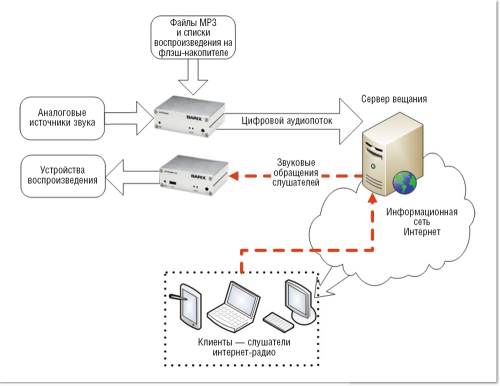
\includegraphics[scale=0.9]{internet_radio}
{\centering\caption{\newline Рис. 1.2.5.1 Схема работы интернет-радио}\\}



\newpage
\chapter{Изучение алгоритмов сжатия данных, в частности, сжатия
аудиоинформации.}
\section{Определение}
\textbf{Сжатие данных} — алгоритмическое обратимое преобразование данных, производимое с целью уменьшения занимаемого ими объёма. Применяется для более рационального использования устройств хранения и передачи данных.
\par Сжатие основано на устранении избыточности, содержащейся в исходных данных. Простейшим примером избыточности является повторение в тексте фрагментов (например, слов естественного или машинного языка). Подобная избыточность обычно устраняется заменой повторяющейся последовательности ссылкой на уже закодированный фрагмент с указанием его длины. Другой вид избыточности связан с тем, что некоторые значения в сжимаемых данных встречаются чаще других. Сокращение объёма данных достигается за счёт замены часто встречающихся данных короткими кодовыми словами, а редких — длинными (энтропийное кодирование). Сжатие данных, не обладающих свойством избыточности (например, случайный сигнал или белый шум, зашифрованные сообщения), принципиально невозможно без потерь.
\section{Принципы сжатия данных}
В основе любого способа сжатия лежит модель источника данных, или, точнее, модель избыточности. Иными словами, для сжатия данных используются некоторые априорные сведения о том, какого рода данные сжимаются. Не обладая такими сведениями об источнике, невозможно сделать никаких предположений о преобразовании, которое позволило бы уменьшить объём сообщения. Модель избыточности может быть статической, неизменной для всего сжимаемого сообщения, либо строиться или параметризоваться на этапе сжатия (и восстановления). Методы, позволяющие на основе входных данных изменять модель избыточности информации, называются адаптивными. Неадаптивными являются обычно узкоспециализированные алгоритмы, применяемые для работы с данными, обладающими хорошо определёнными и неизменными характеристиками. Подавляющая часть достаточно универсальных алгоритмов является в той или иной мере адаптивной.

Все методы сжатия данных делятся на два основных класса:
\begin{itemize}
\item Сжатие без потерь
\item Сжатие с потерями
\end{itemize}
При использовании сжатия без потерь возможно полное восстановление исходных данных, сжатие с потерями позволяет восстановить данные с искажениями, обычно несущественными с точки зрения дальнейшего использования восстановленных данных. Сжатие без потерь обычно используется для передачи и хранения текстовых данных, компьютерных программ, реже — для сокращения объёма аудио- и видеоданных, цифровых фотографий и т. п., в случаях, когда искажения недопустимы или нежелательны. Сжатие с потерями, обладающее значительно большей, чем сжатие без потерь, эффективностью, обычно применяется для сокращения объёма аудио- и видеоданных и цифровых фотографий в тех случаях, когда такое сокращение является приоритетным, а полное соответствие исходных и восстановленных данных не требуется. 
\section{Основные характеристики алгоритмов сжатия}
\subsection{Коэффициент сжатия}
\textbf{Коэффициент сжатия} — основная характеристика алгоритма сжатия. Она определяется как отношение объёма исходных несжатых данных к объёму сжатых данных, то есть: $k = \frac{S_o}{S_c}$, где $k$ - коэффициент сжатия, $S_o$ - объём исходных данных, а $S_c$ - объём сжатых. Таким образом, чем выше коэффициент сжатия, тем алгоритм эффективнее. Следует отметить:
\begin{itemize}
\item если k = 1, то алгоритм не производит сжатия, то есть выходное сообщение оказывается по объёму равным входному;
\item если k < 1, то алгоритм порождает сообщение большего размера, нежели несжатое, то есть, совершает «вредную» работу.
\end{itemize}
\subsection{Допустимость потерь}
Основным критерием различия между алгоритмами сжатия является описанное выше наличие или отсутствие потерь. В общем случае алгоритмы сжатия без потерь универсальны в том смысле, что их применение безусловно возможно для данных любого типа, в то время как возможность применения сжатия с потерями должна быть обоснована. Для некоторых типов данных искажения не допустимы в принципе. В их числе:
\begin{itemize}
\item символические данные, изменение которых неминуемо приводит к изменению их семантики: программы и их исходные тексты, двоичные массивы и т.п.;
\item жизненно важные данные, изменения в которых могут привести к критическим ошибкам: например, получаемые с медицинской измерительной аппаратуры или контрольных приборов летательных, космических аппаратов и т.п.;
\item многократно подвергаемые сжатию и восстановлению промежуточные данные при многоэтапной обработке графических, звуковых и видеоданных.
\end{itemize}
\subsection{Системные требования алгоритмов}
Различные алгоритмы могут требовать различного количества ресурсов вычислительной системы, на которых они реализованы:
\begin{itemize}
\item оперативной памяти (под промежуточные данные);
\item постоянной памяти (под код программы и константы);
\item процессорного времени.

\end{itemize}
В целом, эти требования зависят от сложности и «интеллектуальности» алгоритма. Общая тенденция такова: чем эффективнее и универсальнее алгоритм, тем большие требования к вычислительным ресурсам он предъявляет. Тем не менее, в специфических случаях простые и компактные алгоритмы могут работать не хуже сложных и универсальных. Системные требования определяют их потребительские качества: чем менее требователен алгоритм, тем на более простой, а следовательно, компактной, надёжной и дешёвой системе он может быть реализован.

Так как алгоритмы сжатия и восстановления работают в паре, имеет значение соотношение системных требований к ним. Нередко можно, усложнив один алгоритм, значительно упростить другой. Таким образом, возможны три варианта:
\subsubsection{Алгоритм сжатия требует больших вычислительных ресурсов, нежели алгоритм восстановления.}
Это наиболее распространённое соотношение, характерное для случаев, когда однократно сжатые данные будут использоваться многократно. В качестве примера можно привести цифровые аудио- и видеопроигрыватели.
\subsubsection{Алгоритмы сжатия и восстановления требуют приблизительно равных вычислительных ресурсов.}
Наиболее приемлемый вариант для линий связи, когда сжатие и восстановление происходит однократно на двух её концах (например, в цифровой телефонии).
\subsubsection{Алгоритм сжатия существенно менее требователен, чем алгоритм восстановления.}
Такая ситуация характерна для случаев, когда процедура сжатия реализуется простым, часто портативным, устройством, для которого объём доступных ресурсов весьма критичен, например, космический аппарат или большая распределённая сеть датчиков. Это могут быть также данные, распаковка которых требуется в очень малом проценте случаев, например запись камер видеонаблюдения.
\section{Кодирование аудиоданных}
\subsection{Принципы оцифровки звука}
\textbf{Цифровой звук} — это аналоговый звуковой сигнал, представленный посредством дискретных численных значений его амплитуды.

\textbf{Оцифровка звука} — технология осуществления замеров амплитуды звукового сигнала с определенным временным шагом и последующей записи полученных значений в численном виде.
Другое название оцифровки звука — аналогово-цифровое преобразование звука.

Оцифровка звука включает в себя два процесса:
\begin{itemize}
\item процесс дискретизации (осуществление выборки) сигнала по времени
\item процесс квантования по амплитуде.
\end{itemize}

~

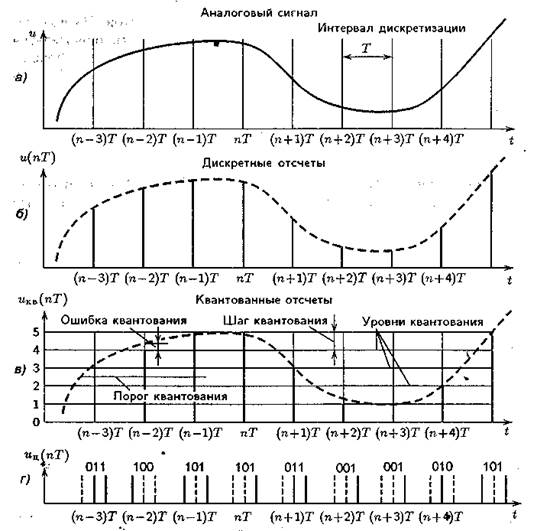
\includegraphics[scale=0.8]{Analog_to_digi}
{\centering\par{Рис. 2.4.1.1 Схема оцифровки звука}\\}

~
\subsubsection{Процесс дискретизации по времени}
\textbf{Процесс дискретизации по времени} — процесс получения значений сигнала, который преобразуется с определенным временным шагом — шагом дискретизации . Количество замеров величины сигнала, осуществляемых в единицу времени, называют частотой дискретизации или частотой выборки. Чем меньше шаг дискретизации, тем выше частота дискретизации и тем более точное представление о сигнале будет получено.
Это подтверждается теоремой Котельникова. Согласно ей, аналоговый сигнал с ограниченным спектром точно описуем дискретной последовательностью значений его амплитуды, если эти значения берутся с частотой, как минимум вдвое превышающей наивысшую частоту спектра сигнала. То есть, аналоговый сигнал, в котором находится частота спектра равная $F_m$, может быть точно представлен последовательностью дискретных значений амплитуды, если для частоты дискретизации $F_d$ выполняется: $F_d>2F_m$.
\par На практике это означает, что для того, чтобы оцифрованный сигнал содержал информацию о всем диапазоне слышимых частот исходного аналогового сигнала (20 Гц — 20 кГц) необходимо, чтобы выбранное значение частоты дискретизации составляло не менее 40 кГц.
\par Основная трудность оцифровки заключается в невозможности записать измеренные значения сигнала с идеальной точностью.
\subsubsection{Линейное квантование амплитуды}
Отведём для записи одного значения амплитуды сигнала в памяти компьютера $N$ бит. Значит, с помощью одного $N$-битного слова можно описать $2N$ разных положений. Пусть амплитуда оцифровываемого сигнала колеблется в пределах от −1 до 1 некоторых условных единиц. Представим этот диапазон изменения амплитуды — \textbf{динамический диапазон сигнала} — в виде $2N−1$ равных промежутков, разделив его на $2N$ уровней — \textbf{квантов}. Теперь, для записи каждого отдельного значения амплитуды, его необходимо округлить до ближайшего уровня квантования. Этот процесс носит название \textbf{квантования по амплитуде}.

\textbf{Квантование по амплитуде} — процесс замены реальных значений амплитуды сигнала значениями, приближенными с некоторой точностью. Каждый из $2^N$ возможных уровней называется \textbf{уровнем квантования}, а расстояние между двумя ближайшими уровнями квантования называется \textbf{шагом квантования}. Если амплитудная шкала разбита на уровни линейно, квантование называют линейным (однородным).
Точность округления зависит от выбранного количества $2N$ уровней квантования, которое, в свою очередь, зависит от количества бит $N$, отведенных для записи значения амплитуды. Число $N$ называют \textbf{разрядностью квантования}, а полученные в результате округления значений амплитуды числа — \textbf{отсчетами} или \textbf{семплами}. Принимается, что погрешности квантования, являющиеся результатом квантования с разрядностью 16 бит, остаются для слушателя почти незаметными. Этот способ оцифровки сигнала — дискретизация сигнала во времени в совокупности с методом однородного квантования — называется \textbf{импульсно-кодовой модуляцией, ИКМ (англ. Pulse Code Modulation — PCM)}.

Оцифрованный сигнал в виде набора последовательных значений амплитуды уже можно сохранить в памяти компьютера. В случае, когда записываются абсолютные значения амплитуды, такой формат записи называется PCM (Pulse Code Modulation). Стандартный аудио компакт-диск (CD-DA), применяющийся с начала 80-х годов, хранит информацию в формате PCM с частотой дискретизации 44.1 кГц и разрядностью квантования 16 бит.  
\subsubsection{Аналогово-Цифровые Преобразователи}
Вышеописанный процесс оцифровки звука выполняется
\textbf{аналогово-цифровыми преобразователями (АЦП)}.
Это преобразование включает в себя следующие операции:
\begin{enumerate}
\item \textbf{Ограничение полосы частот} производится при помощи фильтра нижних частот для подавления спектральных компонент, частота которых превышает половину частоты дискретизации.
\item \textbf{Дискретизация по времени}
\item \textbf{Квантование по уровню}
\item \textbf{Кодирование или оцифровка}, в результате которой значение каждого квантованного отсчета представляется в виде числа, соответствующего порядковому номеру уровня квантования.
\end{enumerate}

\subsection{Кодирование оцифрованного звука}
Для хранения цифрового звука существует много различных способов. Оцифрованный звук являет собой набор значений амплитуды сигнала, взятых через определенные промежутки времени.
\begin{itemize}
\item Блок оцифрованной аудио информации можно записать в файл без изменений, то есть последовательностью чисел — значений амплитуды. В этом случае существуют два способа хранения информации.
\begin{itemize}
\item Первый — PCM (Pulse Code Modulation — импульсно-кодовая модуляция) — способ цифрового кодирования сигнала при помощи записи абсолютных значений амплитуд. (В таком виде записаны данные на всех аудио CD.)
\item Второй — ADPCM (Adaptive Delta PCM — адаптивная относительная импульсно-кодовая модуляция) — запись значений сигнала не в абсолютных, а в относительных изменениях амплитуд (приращениях).
\end{itemize}
\item Можно сжать данные так, чтобы они занимали меньший объем памяти, нежели в исходном состоянии. Тут тоже есть два способа.
\begin{itemize}


\item Кодирование данных без потерь (lossless coding) — способ кодирования аудио, который позволяет осуществлять стопроцентное восстановление данных из сжатого потока. К нему прибегают в тех случаях, когда сохранение оригинального качества данных особо значимо. Существующие сегодня алгоритмы кодирования без потерь (например, Monkeys Audio) позволяют сократить занимаемый данными объем на 20-50\%, но при этом обеспечить стопроцентное восстановление оригинальных данных из полученных после сжатия.
\item Кодирование данных с потерями (lossy coding). Здесь цель — добиться схожести звучания восстановленного сигнала с оригиналом при как можно меньшем размере сжатого файла. Это достигается путём использования алгоритмов, «упрощающих» оригинальный сигнал (удаляющих из него «несущественные», неразличимые на слух детали). Это приводит к тому, что декодированный сигнал перестает быть идентичным оригиналу, а является лишь «похоже звучащим». Методов сжатия, а также программ, реализующих эти методы, существует много. Наиболее известными являются MPEG-1 Layer I,II,III (последним является всем известный MP3), MPEG-2 AAC (advanced audio coding), Ogg Vorbis, Windows Media Audio (WMA), TwinVQ (VQF), MPEGPlus, TAC, и прочие. В среднем, коэффициент сжатия, обеспечиваемый такими кодерами, находится в пределах 10-14 (раз). В основе всех lossy-кодеров лежит использование так называемой психоакустической модели. Она занимается этим самым «упрощением» оригинального сигнала. Степень сжатия оригинального сигнала зависит от степени его «упрощения» — сильное сжатие достигается путём «воинственного упрощения» (когда кодером игнорируются множественные нюансы). Такое сжатие приводит к сильной потере качества, поскольку удалению могут подлежать не только незаметные, но и значимые детали звучания.
\end{itemize}
\end{itemize}

\subsection{Сжатие аудиоданных без потерь}
Сокращение статистической избыточности основано на учёте свойств самих звуковых сигналов. Она определяется наличием корреляционной связи между соседними отсчетами цифрового звукового сигнала, устранение которой позволяет сокращать объём передаваемых данных на 15-25 \% по сравнению с их исходной величиной. Для передачи сигнала необходимо получить более компактное его представление, что возможно осуществить с помощью ортогонального преобразования. Важными условиями применения такого метода преобразования являются:

\begin{itemize}
\item возможность восстанавливать исходный сигнал без искажений
\item способность обеспечивать наибольшую концентрацию энергии в небольшом числе коэффициентов преобразования
\item быстрый вычислительный алгоритм
\end{itemize}
    
Этим требованиям отвечает модифицированное дискретно-косинусное преобразование (МДКП).

Уменьшить скорость цифрового потока позволяют методы кодирования, учитывающие статистику звуковых сигналов, например, вероятности появления уровней разной величины. Одним из таких методов является код Хаффмана, где наиболее вероятным значениям сигнала приписываются более короткие кодовые слова, а значения отсчетов, вероятность появления которых мала, кодируются кодовыми словами большей длины. Именно в силу этих двух причин в наиболее эффективных алгоритмах компрессии цифровых аудиоданных кодированию подвергаются не сами отсчеты звукового сигнала, а коэффициенты МДКП.

Подобные методы применяются при архивации файлов. 


\subsection{Сжатие аудиоданных с потерями}
Сжатие аудиоданных с потерями основывается на несовершенстве человеческого слуха при восприятии звуковой информации. Неспособность человека в определённых случаях различать тихие звуки в присутствии более громких, называемая эффектом маскировки, была использована в алгоритмах сокращения психоакустической избыточности. Эффекты слухового маскирования зависят от спектральных и временных характеристик маскируемого и маскирующего сигналов и могут быть разделены на две основные группы:
\begin{itemize}
\item частотное (одновременное) маскирование
\item временное (неодновременное) маскирование
\end{itemize}
Эффект маскирования в частотной области связан с тем, что в присутствии больших звуковых амплитуд человеческое ухо нечувствительно к малым амплитудам близких частот. То есть, когда два сигнала одновременно находятся в ограниченной частотной области, то более слабый сигнал становится неслышимым на фоне более сильного.

Маскирование во временной области характеризует динамические свойства слуха, показывая изменение во времени относительного порога слышимости (порог слышимости одного сигнала в присутствии другого), когда маскирующий и маскируемый сигналы звучат не одновременно. При этом следует различать явления послемаскировки (изменение порога слышимости после сигнала высокого уровня) и предмаскировки (изменение порога слышимости перед приходом сигнала максимального уровня). Более слабый сигнал становится неслышимым за 5 − 20 мс до включения сигнала маскирования и становится слышимым через 50 − 200 мс после его включения.

Наилучшим методом кодирования звука, учитывающим эффект маскирования, оказывается полосное кодирование. Сущность его заключается в следующем. Группа отсчетов входного звукового сигнала, называемая кадром, поступает на блок фильтров который разделяет сигнал на частотные поддиапазоны. На выходе каждого фильтра оказывается та часть входного сигнала, которая попадает в полосу пропускания данного фильтра. Далее, в каждой полосе с помощью психоакустической модели, анализируется спектральный состав сигнала и оценивается, какую часть сигнала следует передавать без сокращений, а какая лежит ниже порога маскирования и может быть переквантована на меньшее число бит. Для сокращения максимального динамического диапазона определяется максимальный отсчет в кадре и вычисляется масштабирующий множитель, который приводит этот отсчет к верхнему уровню квантования. Эта операция аналогична компандированию в аналоговом вещании. На этот же множитель умножаются и все остальные отсчеты. Масштабирующий множитель передается к декодеру вместе с кодированными данными для коррекции коэффициента передачи последнего. После масштабирования производится оценка порога маскирования и осуществляется перераспределение общего числа битов между всеми полосами.

Очевидно, что после устранения психоакустической избыточности звуковых сигналов их точное восстановления при декодировании оказывается уже невозможным. Методами устранения психофизической избыточности можно обеспечить сжатие цифровых аудиоданных в 10 − 12 раз без существенных потерь в качестве.

\subsection{Структура кодера сжатия аудиоданный с потерями}
\begin{itemize}
\item Исходный цифровой звуковой сигнал разделяется на частотные поддиапазоны и сегментируется по времени в блоке временной и частотной сегментации.
\item Длина кодируемой выборки зависит от формы временной функции звукового сигнала. При отсутствии резких выбросов по амплитуде используется так называемая длинная выборка, обеспечивающая высокое разрешение по частоте. В случае же резких изменений амплитуды сигнала длина кодируемой выборки резко уменьшается, что дает более высокое разрешение по времени. Решение об изменении длины кодируемой выборки принимает блок психоакустического анализа, вычисляя значение психоакустической энтропии сигнала.
\item После сегментации сигналы частотных поддиапазонов нормируются, квантуются и кодируются. В наиболее эффективных алгоритмах компрессии кодированию подвергаются не сами отсчеты выборки звукового сигнала, а соответствующие им коэффициенты МДКП.
\item Учёт закономерностей слухового восприятия звукового сигнала выполняется в блоке психоакустического анализа. Здесь по специальной процедуре для каждого частотного поддиапазона рассчитывается максимально допустимый уровень искажений (шумов) квантования, при котором они ещё маскируются полезным сигналом данного поддиапазона.
\item Блок динамического распределения бит в соответствии с требованиями психоакустической модели для каждого поддиапазона кодирования выделяет такое минимально возможное их количество, при котором уровень искажений, вызванных квантованием, не превышал порога их слышимости, рассчитанного психоакустической моделью.
\item Также могут использоваться:
\begin{itemize}
\item матрицирование стерео — сложение и вычитание левого и правого канала для устранения повторяющейся информации
\item специальные процедуры итерационных циклов, позволяющие управлять величиной энергии искажений квантования в поддиапазонах при недостаточном числе доступных для кодирования бит
\item процедуры линейного и обратного адаптивного предсказаний
\item техника сглаживания переходных шумов во временной области (Temporal Noise Shaping — TNS), позволяющая управлять микроструктурой искажений квантования внутри каждого поддиапазона кодирования
\end{itemize}
\end{itemize}
Многие другие приёмы могут послужить способом сократить объём данных звуковой информации. Даже простое сужение полосы частот сигнала вместе с уменьшением динамического диапазона может уже называться сжатием аудиоданных. Например, в стандарте сжатия звука в сотовой связи используется и то и другое. Стремясь удалить избыточность из звука, кодек при плохом качестве сигнала становится избирателен к определённым словам, упорно проглатывая их. 

\chapter{Изучение алгоритмов блочного и поточного шифрования данных}
\section{Алгоритмы блочного шифрования данных}
\subsection{Определение и основные свойства блочного шифра}
Блочный шифр — разновидность симметричного шифра, оперирующего группами бит фиксированной длины — блоками, характерный размер которых меняется в пределах 64‒256 бит. Если исходный текст (или его остаток) меньше размера блока, перед шифрованием его дополняют. Фактически, блочный шифр представляет собой подстановку на алфавите блоков, которая, как следствие, может быть моно- или полиалфавитной. Блочный шифр является важной компонентой многих криптографических протоколов и широко используется для защиты данных, передаваемых по сети.

Блочный шифр способен зашифровать одним ключом одно или несколько сообщений суммарной длиной больше, чем длина ключа. От поточных шифров работа блочного отличается обработкой бит группами, а не потоком. При этом блочные шифры медленнее поточных. Симметричные системы обладают преимуществом над асимметричными в скорости шифрования, что позволяет им оставаться актуальными, несмотря на более слабый механизм передачи ключа (получатель должен знать секретный ключ, который необходимо передать по уже налаженному зашифрованному каналу. В то же время, в асимметричных шифрах открытый ключ, необходимый для шифрования, могут знать все, и нет необходимости в передаче ключа шифрования).

К достоинствам блочных шифров относят сходство процедур шифрования и расшифрования, которые, как правило, отличаются лишь порядком действий. Это упрощает создание устройств шифрования, так как позволяет использовать одни и те же блоки в цепях шифрования и расшифрования. 
\newpage Гибкость блочных шифров позволяет использовать их для построения других криптографических примитивов: генератора псевдослучайной последовательности, поточного шифра, имитовставки и криптографических хешей.

\subsubsection{Структура блочного шифра}
Блочный шифр состоит из двух парных алгоритмов: шифрования и расшифрования. Оба алгоритма можно представить в виде функций. Функция шифрования E (encryption) на вход получает блок данных M (message) размером n бит и ключ K (key) размером k бит и на выходе отдает блок шифротекста C (cipher) размером n бит:

~

$E_K(M) := E(K,M) : \{0,1\}^k \times \{0,1\}^n \to \{0,1\}^n$.

~

Для любого ключа K, $E_K$ является биективной функцией (перестановкой) на множестве n-битных блоков. Функция расшифрования D (decryption) на вход получает шифротекст C, ключ K и на выходе отдает M:

~

$D_K(C) := D(K,C) : \{0,1\}^k \times \{0,1\}^n \to \{0,1\}^n$,

~

являясь, при этом, обратной к функции шифрования:

~

$D = E^{-1}$,
\medskip

\forall K: $D_K(E_K(M)) = M$
\medskip

$E_K(D_K(C)) = C$.

~

Заметим, что ключ, необходимый для шифрования и дешифрования, один и тот же — следствие симметричности блочного шифра.

\subsection{Алгоритм шифрования DES}
Алгоритм шифрования данных DES (Data Encryption Standard) был опублико­ван в 1977 году. Является официальным стандартом США. Блочный симметричный алгоритм DES пока остается наиболее распространенным алгоритмом, используемым в системах защиты коммерческой информации.

\subsubsection{Принцип работы DES}
Алгоритм DES состоит из чередующейся последовательности перестановок и подстановок. Алгоритм DES осуществляет шифрование 64-битовых блоков данных с помощью 64-битового ключа, в котором значащими являются 56 бит (остальные 8 – проверочные биты для контроля четности).


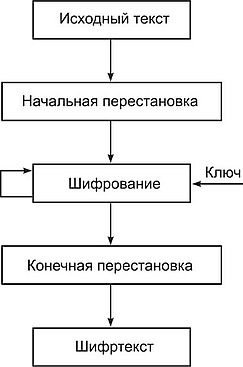
\includegraphics[scale=1.4]{DES}
{\centering\caption{\newline Рис. 3.1.2.1 Обобщенная схема шифрования в алгоритме DES}\\}

~

Процесс шифрования в блочном алгоритме DES (рис. 3.1.2.1) заключается в начальной перестановке битов 64-битового блока, шестнадцати циклах (раундах) шифрования и, наконец, в конечной переста­новке битов. Расшифрование в DES является операцией, обратной шифрованию, и выполняется путем повторения операций шифрования в обратной последовательности.

~

\subsubsection{Процесс зашифрования}
Исходный текст $T$ (блок 64 бит) преобразуется c помощью начальной перестановки $IP$ которая определяется таблицей 3.1.2.1:

~

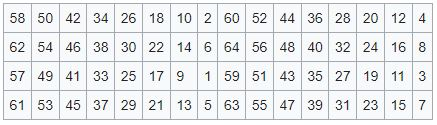
\includegraphics[scale=1.1]{табл}
{\centering\caption{\newline Таблица 3.1.2.1 Начальная перестановка IP}\\}

~

По таблице первые 3 бита результирующего блока $IP(T)$ после начальной перестановкиявляются битами 58, 50, 42 входного блока , а его 3 последние бита являются битами 23, 15, 7 входного блока.

Полученный после начальной перестановки 64-битовый блок $IP(T)$ участвует в 16 циклах преобразования Фейстеля.

Преобразования Фейстеля- это преобразование над векторами (блоками), представляющими собой левую и правую половины регистра сдвига. В алгоритме DES используются прямое преобразование сетью Фейстеля в шифровании и обратное преобразование сетью Фейстеля в расшифровании.

~

16 циклов преобразования Фейстеля:

~

Разбить IP(T) на две части $}L_0, R_0$, где $L_0, R_0$ — соответственно 32 старших битов и 32 младших битов блока $T_{0} IP(T)$ = $L_0 R_0$

Пусть $T_{i-1}=L_{i-1}R_{i-1}$ результат (i-1) итерации, тогда результат i-ой итерации $T_{i}=L_{i}R_{i}$ определяется:

~

$L_i = R_{i-1}$ \\
$R_{i}=L_{i-1}\oplus f(R_{i-1},k_{i})}$ 

~

Левая половина $L_{i}$ равна правой половине предыдущего вектора $L_{i-1}R_{i-1}$.\\ А правая половина $R_i$ — это битовое сложение $L_{i-1}$ и $f(R_{i-1},k_{i})$ по модулю 2.

~

В 16-циклах преобразования Фейстеля функция f играет роль шифрования.

Аргументами функции $f$ являются 32-битовый вектор $R_{i-1}$ и 48-битовый ключ $k_{i}$, который является результатом преобразования 56-битового исходного ключа шифра $k$. Для вычисления функции $f$ последовательно используются

\begin{enumerate}
\item функция расширения $E$
\item сложение по модулю 2 с ключом $k_{i}$
\item преобразование $S$, состоящее из 8 преобразований $S$-блоков ${S} _{1}$,${S} _{2}$,${S} _{3}$\ldots \ ${S} _{8}$
\item перестановка $P$
\end{enumerate}


\subsubsection{Генерирование ключей}
Ключи $k_{i}$ получаются из начального ключа $k$ (56 бит = 7 байтов или 7 символов в ASCII) следующим образом. Добавляются биты в позиции 8, 16, 24, 32, 40, 48, 56, 64 ключа $k$ таким образом, чтобы каждый байт содержал нечетное число единиц. Это используется для обнаружения ошибок при обмене и хранении ключей. Затем делают перестановку для расширенного ключа (кроме добавляемых битов 8, 16, 24, 32, 40, 48, 56, 64).

\subsubsection{Процесс расшифрования}
При расшифровании данных все действия выполняются в обратном порядке. В 16 циклах расшифрования, в отличие от шифрования c помощью прямого преобразования сетью Фейстеля, здесь используется обратное преобразование сетью Фейстеля.

~

$R_{i-1} = L_i$ \\
$L_{i-1} = R_i \oplus f(L_i,k_i)$

~

Ключ $k_{i}$, i=16,…,1, функция f, перестановка IP и $IP^{-1}$ такие же, как и в процессе шифрования. Алгоритм генерации ключей зависит только от ключа пользователя, поэтому при расшифровании они идентичны.


\subsubsection{Режимы использования DES}
DES может использоваться в четырёх режимах.

\begin{enumerate}
\item Режим электронной кодовой книги (ECB — Electronic Codebook): обычное использование DES как блочного шифра. Шифруемый текст разбивается на блоки, при этом каждый блок шифруется отдельно, не взаимодействуя с другими блоками (см. рис. 3.1.2.2)

~

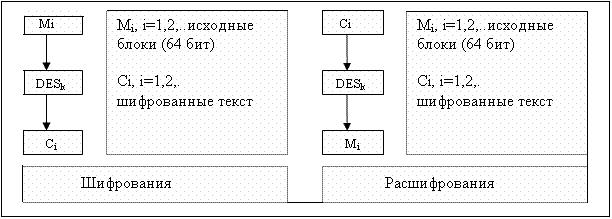
\includegraphics[scale=1.2]{ECB1}
{\centering\caption{\newline Рис. 3.1.2.2 Режим электронной кодовой книги — ECB}\\}

~


\item Режим сцепления блоков шифротекста (СВС — Cipher Block Chaining)(см. рис. 3.1.2.3). Каждый очередной блок $M_{i}$ i>=1, перед зашифровыванием складывается по модулю 2 с предыдущим блоком зашифрованного текста $C_{i-1}$. Вектор $C_{0}$ — начальный вектор, он меняется ежедневно и хранится в секрете.

~

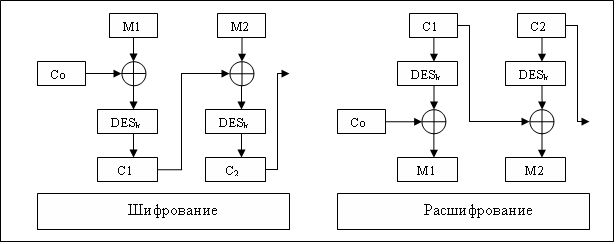
\includegraphics[scale=1.1]{CBC}
{\centering\caption{\newline Рис. 3.1.2.3 Режим сцепления блоков — СВС}\\}

~

\item Режим обратной связи по шифротексту (Cipher Feedback) (см. рис. 3.1.2.4). В режиме CFB вырабатывается блочная «гамма» $Z_{0},Z_{1},...,Z_{i}=DES_{k}(C_{i-1})$ $C_{i} = M_{i}\oplus Z_{i}$. Начальный вектор $C_{0}$ является синхропосылкой и предназначен для того, чтобы разные наборы данных шифровались по-разному с использованием одного и того же секретного ключа. Синхропосылка посылается получателю в открытом виде вместе с зашифрованным файлом. Алгоритм DES, в отличие от предыдущих режимов, используется только как шифрование (в обоих случаях).

~

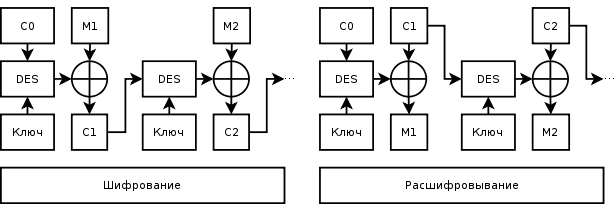
\includegraphics[scale=0.7]{CF}
{\centering\caption{\newline Рис.3.1.2.4 Режим обратной связи по шифротексту — CFB}\\}

~

\item Режим обратной связи по выходу (Output Feedback) (см. Рис. 3.1.2.5). В режиме OFB вырабатывается блочная «гамма» $Z_{0},Z_{1},...,Z_{i}=DES_{k}(Z_{i-1})C_{i}=M_{i}\oplus Z_{i}$ , i>=1. Режим также использует DES только как шифрование (в обоих случаях).

~

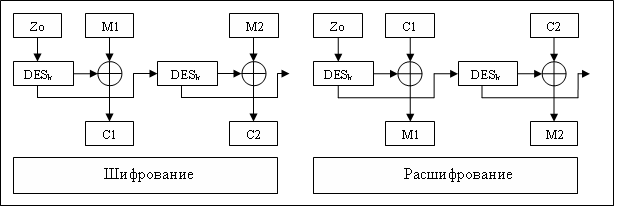
\includegraphics[scale=1.1]{OFB}
{\centering\caption{\newline Рис. 3.1.2.5 Режим обратной связи по выходу — OFB}\\}
\end{enumerate}






\subsubsection{Достоинства и недостатки DES}
Основные достоинства алгоритма шифрования DES:
\begin{itemize}
\item относительная простота алгоритма обеспечивает высокую скорость\\ обработки;
\item для расшифровки сообщения, зашифрованного с помощью одного пакета программ, можно использовать любой другой пакет программ, соответствующий алгоритму DES;
\item криптостойкость алгоритма достаточна для защиты коммерческой \\ информации.
\end{itemize}

Также алгоритм DES имеет ряд существенных недостатков. Основные из них 
\begin{itemize}
\item битовые операции в узлах замены неэффективно реализуются программ­ным путем;
\item  короткая длина ключа (56 битов), что помогает организо­вать полный перебор;
\end{itemize}

\subsection{Алгоритм шифрования IDEA}
IDEA (англ. International Data Encryption Algorithm, международный алгоритм шифрования данных) — cимметричный блочный алгоритм шифрования данных, запатентованный швейцарской фирмой Ascom. Известен тем, что применяется в пакете программ шифрования PGP и в его свободной альтернативе GnuPG.

Первую версию алгоритма разработали в 1990 году Сюэцзя Лай и Джеймс Мэсси из Швейцарского института ETH Zürich в качестве замены DES и назвали ее PES (англ. Proposed Encryption Standard, предложенный стандарт шифрования). Затем, после публикации работ Бихама и Шамира по дифференциальному криптоанализу PES, алгоритм был улучшен с целью усиления криптостойкости и назван IPES (англ. Improved Proposed Encryption Standard, улучшенный предложенный стандарт шифрования). Через год его переименовали в IDEA.

\subsubsection{Принцип работы}

IDEA использует 128-битный ключ и 64-битный размер блока. Открытый текст разбивается на блоки по 64 бит, если такое разбиение невозможно, используются различные режимы шифрования.Каждый исходный незашифрованный 64-битный блок делится на четыре подблока по 16 бит каждый, так как все алгебраические операции, использующиеся в процессе шифрования, совершаются над 16-битными числами. Для шифрования и расшифрования IDEA использует один и тот же алгоритм.

~

Фундаментальным нововведением в алгоритме является использование операций из разных алгебраических групп, а именно:
\begin{itemize}
\item сложение по модулю $2^{16}$
\item умножение по модулю $2^{16}+1$
\item побитовое исключающее ИЛИ (XOR).
\end{itemize}

~

Эти три операции несовместимы в том смысле, что:
\begin{itemize}
\item никакие две из них не удовлетворяют дистрибутивному закону, то есть \\ $a*(b+c)\ <>\ (a*b)+(a*c)$
\item никакие две из них не удовлетворяют ассоциативному закону, то есть \\ $a+(b\oplus c)\ <>\ (a+b)\oplus c$
\end{itemize}

~

Применение этих трех операций затрудняет криптоанализ IDEA по сравнению с DES, который основан исключительно на операции исключающее ИЛИ, а также позволяет отказаться от использования S-блоков и таблиц замены. IDEA является модификацией сети Фейстеля.

\subsubsection{Шифрование}

Процесс шифрования состоит из восьми одинаковых раундов шифрования и одного выходного преобразования. Исходный незашифрованный текст делится на блоки по 64 бита. Каждый такой блок делится на четыре подблока по 16 бит каждый. На рисунке эти подблоки обозначены $D_{1}$, $D_{2}$, $D_{3}$, $D_{4}$. В каждом раунде используются свои подключи согласно таблице подключей. Над 16-битными подключами и подблоками незашифрованного текста производятся следующие операции:



\begin{itemize}
\item умножение по модулю $2^{16}+1} = 65537$, причем вместо нуля используется $2^{16}$
\item сложение по модулю $2^{16}$
\item побитовое исключающее ИЛИ
\end{itemize}

В конце каждого раунда шифрования имеется четыре 16-битных подблока, которые затем используются как входные подблоки для следующего раунда шифрования. Выходное преобразование представляет собой укороченный раунд, а именно, четыре 16-битных подблока на выходе восьмого раунда и четыре соответствующих подключа подвергаются операциям:

\begin{itemize}
\item умножение по модулю $2^{16}+1}$
\item сложение по модулю $2^{16}$
\end{itemize}

После выполнения выходного преобразования конкатенация подблоков $D_{1}'$, $D_{2}'$, $D_{3}'$ и $D_{4}'$ представляет собой зашифрованный текст. Затем берется следующий 64-битный блок незашифрованного текста и алгоритм шифрования повторяется. Так продолжается до тех пор, пока не зашифруются все 64-битные блоки исходного текста.

Структура алгоритма IDEA показана на рисунке 3.1.3.1.

~

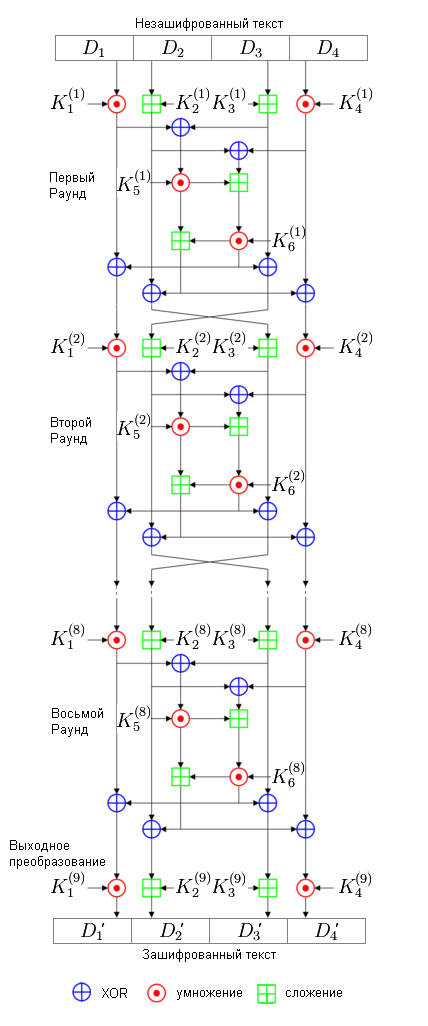
\includegraphics[scale=0.7]{IDEA_encryption}
{\centering\caption{\newline Рис. 3.1.3.1 Схема шифрования IDEA}\\}

\subsubsection{Расшифровка}
Метод вычисления, использующийся для расшифровки текста по существу такой же, как и при его шифровании. Единственное отличие состоит в том, что для расшифровки используются другие подключи.

В процессе расшифровки подключи должны использоваться в обратном порядке. Первый и четвёртый подключи i-го раунда расшифровки получаются из первого и четвёртого подключа (10-i)-го раунда шифрования мультипликативной инверсией. Для 1-го и 9-го раундов второй и третий подключи расшифровки получаются из второго и третьего подключей 9-го и 1-го раундов шифрования аддитивной инверсией. Для раундов со 2-го по 8-й второй и третий подключи расшифровки получаются из третьего и второго подключей с 8-го по 2-й раундов шифрования аддитивной инверсией. Последние два подключа i-го раунда расшифровки равны последним двум подключам (9-i)-го раунда шифрования.

Мультипликативная инверсия подключа K обозначается 1/K и $(1/K)*K=1\ mod\ (2^{16}+1)$. Так как $2^{16}+1$ — простое число, каждое целое не равное нулю K имеет уникальную мультипликативную инверсию по модулю $2^{16}+1}$. Аддитивная инверсия подключа K обозначается -K и $-K+K=0\ mod\ (2^{16})$.

\subsubsection{Достоинства и недостатки IDEA}
Преимущества алгоритма IDEA:

\begin{itemize}
\item В программной реализации на Intel486SX по сравнению с DES IDEA в два раза быстрее, что является существенным повышением скорости, длина ключа у IDEA имеет размер 128 бит, против 56 бит у DES, что является хорошим улучшением против полного перебора ключей;
\item Использование IDEA в параллельных режимах шифрования на процессорах Pentium III и Pentium MMX позволяет получать высокие скорости;
\item  Хорошая изученность и устойчивость к общеизвестным средствам криптоанализа.
\end{itemize}

Недостатки алгоритма IDEA:

\begin{itemize}
\item IDEA значительно медленнее, почти в два раза, чем Blowfish;
\item IDEA не предусматривает увеличение длины ключа.
\end{itemize}



\subsection{Алгоритм шифрования RC5}
RC5 (Ron’s Code 5 или Rivest’s Cipher 5) — это блочный шифр, разработанный Роном Ривестом из компании RSA Security с переменным количеством раундов, длиной блока и длиной ключа.
Он отличается простотой, быстротой (за счет использования только примитивных компьютерных операций, таких как XOR, shift и т. Д.) И использует меньше памяти.
Это расширяет сферу использования и упрощает переход на более сильный вариант алгоритма. 



Существует несколько различных вариантов алгоритма, в которых преобразования в «пол-раундах» классического RC5 несколько изменены. В классическом алгоритме используются три примитивных операции и их инверсии:
\begin{itemize}

\item сложение по модулю $\displaystyle 2^{w}$
\item побитовое исключающее ИЛИ (XOR)
\item операции циклического сдвига на переменное число бит $(x \lll y).$
\end{itemize}

Основным нововведением является использование операции сдвига на переменное число бит, не использовавшиеся в более ранних алгоритмах шифрования. Эти операции одинаково быстро выполняются на большинстве процессоров, но в то же время значительно усложняют дифференциальный и линейный криптоанализ алгоритма.

Шифрование по алгоритму RC5 состоит из двух этапов. Процедура расширения ключа и непосредственно шифрование. Для расшифрования выполняется сначала процедура расширения ключа, а затем операции, обратные процедуре шифрования. Все операции сложения и вычитания выполняются по модулю $\displaystyle 2^{w}$. 

\subsubsection{Параметры алгоритма}
Так как алгоритм RC5 имеет переменные параметры, то для спецификации алгоритма с конкретными параметрами принято обозначение \textbf{RC5-W/R/b}, где:
\begin{itemize}
\item W — половина длины блока в битах, возможные значения 16, 32 и 64. Для эффективной реализации величину W рекомендуют брать равным машинному слову. Например, для 32-битных платформ оптимальным будет выбор W=32, что соответствует размеру блока 64 бита.
\item R — число раундов, возможные значения от 0 до 255. Увеличение числа раундов обеспечивает увеличение уровня безопасности шифра. Так, при R=0 информация шифроваться не будет. Также алгоритм RC5 использует таблицу расширенных ключей размера $\displaystyle 2(R+1)$ слов, которая получается из ключа заданного пользователем.
\item b — длина ключа в байтах, возможные значения от 0 до 255.
\end{itemize} 


\subsubsection{Расширение ключа}
Перед непосредственно шифрованием или расшифрованием данных выполняется процедура расширения ключа. Процедура генерации ключа состоит из четырёх этапов: 

\begin{itemize}

\item Генерация констант
\item Разбиение ключа на слова
\item Построение таблицы расширенных ключей
\item Перемешивание

\end{itemize}

\textbf{Генерация констант}

Для заданного параметра $W$ генерируются две псевдослучайные величины используя две математические константы: $e$ (экспонента) и $f$ (Золотое сечение).

$Q_w \leftarrow \textrm{Odd}((f − 1)\cdot 2^w)$

$P_w \leftarrow \textrm{Odd}((e − 2)\cdot 2^w)$

$\textrm{Odd()}$ - округление до ближайшего нечетного целого.

~

\textbf{Разбиение ключа на слова}

На этом этапе происходит копирование ключа $K_0 … K_{b − 1}$ в массив слов $L_0… L_{c − 1}$, где $c = b / u$, где $u = W / 8$, то есть, количество байт в слове.

Если $b$ не кратен $W / 8$, то $L$ дополняется нулевыми битами до ближайшего большего размера $c$, кратного $W / 8$.

В случае если $b = c = 0$, то мы устанавливаем значение $c = 1$, а $L_0 = 0$.

~

\textbf{Построение таблицы расширенных ключей}

На этом этапе происходит построение таблицы расширенных ключей $S_0 … S_{2 ∗ ( R + 1 ) − 1}$, которое выполняется следующим образом: 

$S_{0}=P_{w}$

$S_{i+1}=S_i+Q_w$

~

\textbf{Перемешивание}

Циклически N раз выполняются следующие действия:

${\displaystyle G=S_{i}=(S_{i}+G+H)\lll 3}$

${\displaystyle H=L_{j}=(L_{j}+G+H)\lll (G+H)}$

${\displaystyle i=(i+1)\mod (2(R+1))}$

${\displaystyle j=(j+1)\mod c}$,

$G, H, i, j$ — временные переменные, начальные значения которых равны 0. Количество итераций цикла N — это максимальное из двух значений $3 ∗ c$ и $(3 \cdot 2 \cdot (R + 1))$ 

\subsubsection{Шифрование}
Перед первым раундом выполняются операции наложения расширенного ключа на шифруемые данные:

$A=(A+S_0) \bmod {2^{w}}$

$B=(B+S_1)\bmod {2^{w}}$

В каждом раунде выполняются следующие действия: 

$A=((A\oplus B)\lll B)+S_{2i}$

$B=((B\oplus A)\lll A)+S_{2i+1}$

\subsubsection{Расшифрование}

Для Расшифрования данных используются обратные операции, то есть для $i = R, R − 1,...,1$ выполняются следующие раунды:

$B=((B-S_{2i+1})\ggg A)\oplus A$

$A=((A-S_{2i})\ggg B)\oplus B$

После выполнения всех раундов, исходное сообщение находится из выражения: 

$B=(B-S_1)\bmod {2^{w}}$

$A=(A-S_0)\bmod {2^{w}}$


\section{Алгоритмы поточного шифрования данных}
\subsection{Определение и основные свойства поточного шифра}
Поточный или потоковый шифр — это симметричный шифр, в котором каждый символ открытого текста преобразуется в символ шифрованного текста в зависимости не только от используемого ключа, но и от его расположения в потоке открытого текста. Поточный шифр реализует другой подход к симметричному шифрованию, нежели блочные шифры (тот же принцип и для шифрования аудиоданных).

Характерной особенностью поточных шифров есть побитная обработка информации. При этом шифрование и дешифрование может обрыватся в произвольный момент времени. И как только связь восстановлена можно продолжать процедуру без проблем.

~

Поточные шифры называют шифрами гаммирования. Также само шифрование есть методом защиты информации. Эти шифры в разы быстрее своих конкурентов — блочных шифров, если оно реализовано аппаратно. Если же реализация программная, здесь скорость может быть даже меньше блоковых шифров. Функция которая формирует гамму, руководствуется тремя компонентами: 

\begin{itemize}
\item ключ;
\item номер текущего шага шифрования;
\item ближние биты исходного или зашифрованного текста от текущей позиции.
\end{itemize}

\newpage
На рисунке 3.2.1.1 представлен режим гаммирования потоковых шифров.

~

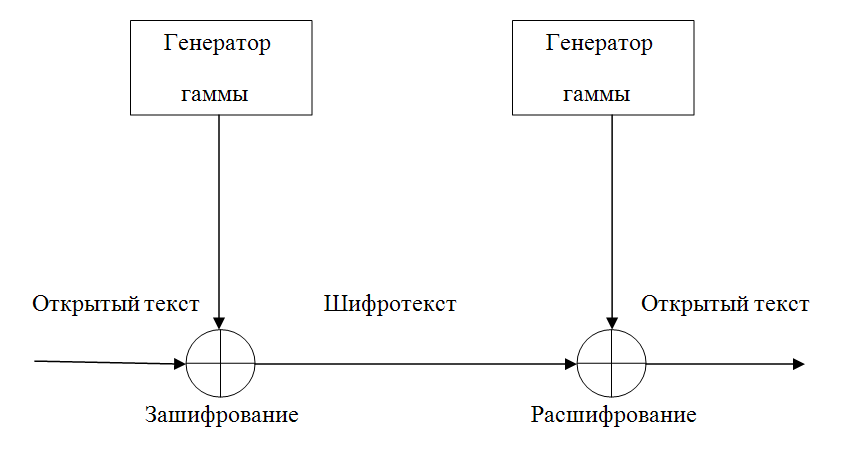
\includegraphics[scale=0.5]{Gamma12}
{\centering\caption{\newline Рис. 3.2.1.1 Режим гаммирования для поточных шифров}\\}



\subsubsection{Классификация потоковых шифров}
Для предотвращения потери информации решают проблему синхронизации шифрования и расшифрования текста.
По способу решения этой проблемы шифросистемы подразделяются на синхронные и системы с самосинхронизацией.

~

\textbf{Синхронные потоковые шифры}

Синхронные потоковые шифры (СПШ) — шифры, в которых поток ключей генерируется независимо от открытого текста и шифротекста.

При шифровании генератор потока ключей выдаёт биты потока ключей, которые идентичны битам потока ключей при дешифровании. Потеря знака шифротекста приведёт к нарушению синхронизации между этими двумя генераторами и невозможности расшифрования оставшейся части сообщения. Очевидно, что в этой ситуации отправитель и получатель должны повторно синхронизоваться для продолжения работы.

Обычно синхронизация производится вставкой в передаваемое сообщение специальных маркеров. В результате этого пропущенный при передаче знак приводит к неверному расшифрованию лишь до тех пор, пока не будет принят один из маркеров.

~

\textbf{Самосинхронизирующиеся потоковые шифры}

Самосинхронизирующиеся потоковые шифры (асинхронные потоковые шифры (АПШ)) — шифры, в которых ключевой поток создаётся функцией ключа и фиксированного числа знаков шифротекста.

Внутреннее состояние генератора потока ключей является функцией предыдущих N битов шифротекста. Поэтому расшифрующий генератор потока ключей, приняв N битов, автоматически синхронизируется с шифрующим генератором.

Реализация этого режима происходит следующим образом: каждое сообщение начинается случайным заголовком длиной N битов; заголовок шифруется, передаётся и расшифровывается; расшифровка является неправильной, зато после этих N бит оба генератора будут синхронизированы


\subsection{Алгоритм шифрования RC4}

RC4 (Rivest cipher 4 или Ron’s code), также известен как ARC4 или ARCFOUR) — потоковый шифр, широко применяющийся в различных системах защиты информации в компьютерных сетях (например, в протоколах SSL и TLS, алгоритмах обеспечения безопасности беспроводных сетей WEP и WPA).

Алгоритм RC4 строится на основе генератора псевдослучайных битов. На вход генератора записывается ключ, а на выходе читаются псевдослучайные биты. Длина ключа может составлять от 40 до 2048 бит. Генерируемые биты имеют равномерное распределение. Генерируемые биты имеют равномерное распределение.

\subsubsection{Принцип работы} 
Ядро алгоритма поточных шифров состоит из функции — генератора псевдослучайных битов (гаммы), который выдаёт поток битов ключа (ключевой поток, гамму, последовательность псевдослучайных битов).

~

\textbf{Алгоритм шифрования}
\begin{enumerate}
\item Функция генерирует последовательность битов $k_{i}$;
\item Затем последовательность битов посредством операции «суммирование по модулю два» (xor) объединяется с открытым текстом $m_{i}$. В результате получается шифрограмма $c_{i}$: $c_{i}=m_{i}\oplus k_{i}$.
\end{enumerate}

~

\textbf{Алгоритм расшифровки}
\begin{enumerate}
\item Повторно создаётся (регенерируется) поток битов ключа (ключевой поток) $k_{i}$;
\item Поток битов ключа складывается с шифрограммой $c_{i}$ операцией «xor». В силу свойств операции «xor» на выходе получается исходный (незашифрованный) текст $m_{i}$:
$m_{i}=c_{i}\oplus k_{i}=(m_{i}\oplus k_{i})\oplus k_{i}$
\end{enumerate}

~

RC4 — фактически класс алгоритмов, определяемых размером блока (в дальнейшем S-блока). Параметр n является размером слова для алгоритма и определяет длину S-блока. Обычно, n = 8, но в целях анализа можно уменьшить его. Однако для повышения безопасности необходимо увеличить эту величину. В алгоритме нет противоречий на увеличение размера S-блока . При увеличении n, допустим, до 16 бит, элементов в S-блоке становится 65 536 и соответственно время начальной итерации будет увеличено. Однако, скорость шифрования возрастёт.

Внутреннее состояние RC4 представляется в виде массива размером 2n и двух счётчиков. Массив известен как S-блок, и далее будет обозначаться как S. Он всегда содержит перестановку 2n возможных значений слова. Два счётчика обозначены через i и j.

Инициализация RC4 состоит из двух частей:
\begin{enumerate}
\item инициализация S-блока;
\item генерация псевдослучайного слова K.
\end{enumerate}

\textbf{Инициализация S-блока}

Алгоритм также известен как «key-scheduling algorithm» или «KSA». Этот алгоритм использует ключ, подаваемый на вход пользователем, сохранённый в Key, и имеющий длину L байт. Инициализация начинается с заполнения массива S, далее этот массив перемешивается путём перестановок, определяемых ключом. Так как только одно действие выполняется над S, то должно выполняться утверждение, что S всегда содержит один набор значений, который был дан при первоначальной инициализации (S[i] := i).

\begin{alltt}
		for i from 0 to 255
    		S[i] := i
		endfor
		j := 0
		for i from 0 to 255
    		j := ( j + S[i] + Key[ i mod L ] ) mod 256
		endfor
\end{alltt}




\textbf{Генерация псевдослучайного слова K}

Эта часть алгоритма называется генератором псевдослучайной последовательности (англ. pseudo-random generation algorithm, PRGA). Генератор ключевого потока RC4 переставляет значения, хранящиеся в S. В одном цикле RC4 определяется одно n-битное слово K из ключевого потока. В дальнейшем ключевое слово будет сложено по модулю два с исходным текстом, которое пользователь хочет зашифровать, и получен зашифрованный текст.

\begin{alltt}
		i := 0
		j := 0
		while GenCycle:
    			i := ( i + 1 ) mod 256
    			j := ( j + S[i] ) mod 256
    			t := ( S[i] + S[j] ) mod 256
    			K := S[t] 
		endwhile
\end{alltt}

\newpage
\subsection{Алгоритм шифрования VMPC}
VMPC (Variably Modified Permutation Composition) — это потоковый шифр, применяющийся в некоторых системах защиты информации в компьютерных сетях. Шифр разработан криптографом Бартошем Жултаком в качестве усиленного варианта популярного шифра RC4. Алгоритм VMPC строится как и любой потоковый шифр на основе параметризованного ключом генератора псевдослучайных битов. Основные преимущества шифра, как и RC4 — высокая скорость работы, переменный размер ключа и вектора инициализации (от 128 до 512 бит включительно), простота реализации (буквально несколько десятков строк кода).

Основа шифра - генератор псевдослучайных чисел, базой которого является односторонняя необратимая функция VMPC.

\subsubsection{Приницип работы}

\textbf{Ключевое расписание}

Алгоритм преобразования ключа и (дополнительно) вектора инициализации в 256-элементную перестановку P. Инициализация глобальной переменной s.

~

С : Длина ключа в байтах $(16\leq c\leq 64)$ 

K : Ключ 

z : Длина вектора инициализации в байтах $(16\leq z\leq 64)$ 

V : Вектор инициализации 

i : 8-разрядная переменная 

j : 16-разрядная переменная 

s : 8-разрядная глобальная переменная 

P : таблица из 256 байт для хранения перестановок 

\begin{alltt}
1.  s = 0
2.  for i = 0 to 255: P[i] = i

3.  for j = 0 to 767 
	4.  i = j mod 256
	5.  s = P[(s + P[i] + K[j mod c]) mod 256]
	6.  Temp = P[i]
  	    P[i] = P[s]
  	    P[s] = Temp
	for j = 0 to 767 
7.  i = j mod 256
8.  s = P[(s + P[i] + V[j mod z]) mod 256]
9. Temp = P[i]
    P[i] = P[s]
    P[s] = Temp
\end{alltt}
 
~

\textbf{Алгоритм зашифрования}

Генерация выходной ключевой последовательности.
Для генерации L байт выходного ключевого потока выполняются следующие операции: 

L : длина ключевой последовательности в байтах

\begin{alltt}
1. i = 0
	3. s = P[(s + P[i]) mod 256]
	4. Output = P[(P[P[s]] + 1) mod 256]
	5. Temp = P[i]
  	   P[i] = P[s]
  	   P[s] = Temp
	6. i = (i + 1) mod 256
\end{alltt}

\subsubsection{Особенности алгоритма VMPC}
Вероятность получения двух последовательных одинаковых результатов при генерации ключевой последовательности при использовании шифра VMPC равна $2^{-N}$ что совпадает с соответствующей вероятностью идеального генератора случайной последовательности.  $N$ -  число разрядов внутреннего состояния генератора псевдослучайной последовательности, обычно равно $8$. В 2005 году А. Максимов показал, что на основании $2^{40}$ выходных бит возможно отличить последовательность генератора VMPC от случайного потока.

 Эксперименты, проведенные Б.Жултаком, показали, что не наблюдается статистически значимого отклонения вероятности появления в выходной последовательности:
\begin{itemize}
\item каждого из возможных $2^{8}$  значений $P=1/256$  для $2^{41.85}$  байт выходной последовательности);
\item каждой из возможных $2^{16}$ пар последовательных значений $P=1/65536$ для $2^{40.1}$ байт выходной последовательности);
\item каждой из возможных $2^{24}$ троек последовательных значений $P=1/16777216$ для $2^{41.6}$ байт выходной последовательности)
\end{itemize}

\subsection{Алгоритм шифрования А5}

А5 — это поточный алгоритм шифрования, используемый для обеспечения конфиденциальности передаваемых данных между телефоном и базовой станцией в европейской системе мобильной цифровой связи GSM (Groupe Spécial Mobile).

Шифр основан на побитовом сложении по модулю два (булева операция «исключающее или») генерируемой псевдослучайной последовательности и шифруемой информации. В A5 псевдослучайная последовательность реализуется на основе трёх линейных регистров сдвига с обратной связью. Регистры имеют длины 19, 22 и 23 бита соответственно. Сдвигами управляет специальная схема, организующая на каждом шаге смещение как минимум двух регистров, что приводит к их неравномерному движению. Последовательность формируется путём операции «исключающее или» над выходными битами регистров.

\subsubsection{Принцип работы}
Алгоритм A5 в настоящее время — это целое семейство шифров. Для описания возьмем А5/1 как родоначальника этого семейства.

~

\textbf{Потоковое шифрование}
В этом алгоритме каждому символу открытого текста соответствует символ шифротекста. Текст не делится на блоки (как в блочном шифровании) и не изменяется в размере. Для упрощения аппаратной реализации и, следовательно, увеличения быстродействия используются только простейшие операции: сложение по модулю 2 (XOR) и сдвиг регистра.

Формирование выходной последовательности происходит путём сложения потока исходного текста с генерируемой последовательностью (гаммой). Особенность операции XOR заключается в том, что применённая чётное число раз, она приводит к начальному значению. Отсюда, декодирование сообщения происходит путём сложения шифротекста с известной последовательностью.

В реальных системах создаётся ключ заданного размера, который без труда передаётся по закрытому каналу. Последовательность генерируется на его основе и является псевдослучайной. Большой класс поточных шифров (в том числе A5) составляют шифры, генератор псевдослучайной последовательности которой основан на регистрах сдвига с линейной обратной связью.

~

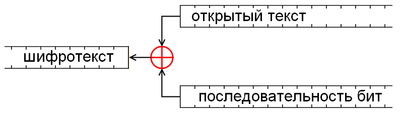
\includegraphics[scale=1.1]{Поточный_шифр}
{\centering\caption{\newline Рис. 3.2.4.1 Схема поточного шифра: сложение открытого текста и последовательности бит даёт шифротекст}\\}

~

\textbf{Система РСЛОС в А5}

Регистр сдвига с линейной обратной связью состоит из собственно регистра (последовательности бит заданной длины) и обратной связи. На каждом такте происходит следующие действия: крайний левый бит (старший бит) извлекается, последовательность сдвигается влево и в опустевшую правую ячейку (младший бит) записывается значение функции обратной связи. Эта функция является суммированием по модулю два определённых битов регистра и записывается в виде многочлена, где степень указывает номер бита. Извлечённые биты формируют выходную последовательность.

~

Сам по себе РСЛОС легко поддаётся криптоанализу и не является достаточно надёжным для использования в шифровании. Практическое применение имеют системы регистров переменного тактирования с различными длинами и функциями обратной связи.

Структура алгоритма А5 выглядит следующим образом:
\begin{itemize}
\item Три регистра(R1, R2, R3) имеют длины 19, 22 и 23 бита,
\item Многочлены обратных связей:
\begin{itemize}
\item $X^{19} + X^{18} + X^{17} + X^{14} + 1$ для R1,
\item $X^{22} + X^{21} + 1$ для R2 и
\item $X^{23} + X^{22} + X^{21} + X^8 + 1$ для R3,
\end{itemize}
\item Управление тактированием осуществляется специальным механизмом:
\begin{itemize}
\item в каждом регистре есть биты синхронизации: 8 (R1), 10 (R2), 10 (R3),
\item вычисляется функция $F = x\&y|x\&z|y\&z$, где \& — булево AND, | - булево OR, а x, y и z — биты синхронизации R1, R2 и R3 соответственно,
\item сдвигаются только те регистры, у которых бит синхронизации равен F,
\item фактически, сдвигаются регистры, синхробит которых принадлежит большинству,
\end{itemize}
\item Выходной бит системы — результат операции XOR над выходными битами регистров.
\end{itemize}

\textbf{Функционирование алгоритма}

Рассмотрим особенности функционирования алгоритма на основе известной схемы. Передача данных осуществляется в структурированном виде — с разбивкой на кадры (114 бит). Перед инициализацией регистры обнуляются, на вход алгоритма поступают сеансовый ключ (K — 64 бита), сформированный А8, и номер кадра (Fn — 22 бита). Далее последовательно выполняются следующие действия:

\begin{itemize}
\item Инициализация:
\begin{itemize}
\item 64 такта, при которых очередной бит ключа XOR-ится с младшим битом каждого регистра, регистры при этом сдвигаются на каждом такте,
\item аналогичные 22 такта, только операция XOR производится с номером кадра,
\item 100 тактов с управлением сдвигами регистров, но без генерации последовательности,
\end{itemize}
\item $228 (114 + 114)$ тактов рабочие, происходит шифрование передаваемого кадра (первые 114 бит) и дешифрование (последние 114 бит) принимаемого,
\item далее инициализация производится заново, используется новый номер кадра.
\end{itemize}


\newpage
\begin{thebibliography}{}
\bibitem{} https://ru.wikipedia.org
\bibitem{} https://www.sviaz-expo.ru/ru/ui/17142/
\bibitem{} https://www.osp.ru/nets/1996/07/141827
\bibitem{} http://asvagroup.com/2020/12/rasprostranenie-radiovoln-v-srede-i-peredacha-dannyh/
\bibitem{} http://www.comprice.ru/articles/detail.php?ID=40210
\bibitem{} https://ru.wikipedia.org/wiki/Сжатие\_данных
\bibitem{} https://ru.wikipedia.org/wiki/Кодирование\_звуковой\_информации

\end{thebibliography}











\end{document}





